This \cgal\ package provides functions to compute global informations
on the shape of a set of 2D or 3D objects such as points. It provides the computation of axis-aligned bounding boxes, centroids of point sets, barycenters of weighted point sets, as well as linear least squares fitting for point sets in 2D, and point sets as well as triangle sets in 3D. The sets are specified by iterator ranges of containers.\\

\section{Definitions}

A \emph{bounding box} for a set of objects is a cuboid that completely
contains the set. An \emph{axis-aligned bounding box} is a bounding box
aligned with the axes of the coordinate system.\\

A \emph{centroid} is defined as average of position. A \emph{barycenter} of weighted point sets is defined as weighted average of position. When all weights are equal the barycenter coincides with the centroid.\\

Given a point set, \emph{linear least squares fitting} amounts to
find the linear sub-space which minimizes the sum of squared
distances from the points to their projection onto this linear
sub-space. This problem is equivalent to search for the linear
sub-space which maximizes the variance of projected points, the latter
being obtained by eigen decomposition of the covariance
matrix of the point set. Eigenvectors corresponding to large eigenvalues are the
directions in which the data has strong component, or equivalently
large variance. If eigenvalues are the same there is no preferable
sub-space.\\

Given a triangle set, \emph{linear least squares fitting} amounts to find the linear sub-space which minimizes the sum of squared
distances from all points in the set to their projection onto this linear
sub-space. This problem is equivalent to the one of fitting a linear sub-space to a point set, except that the covariance matrix is now derived from a continuous integral over the triangles instead of a discrete sum over the points.


\begin{center}
    \label{fit}
    % Image
    \begin{ccTexOnly}
      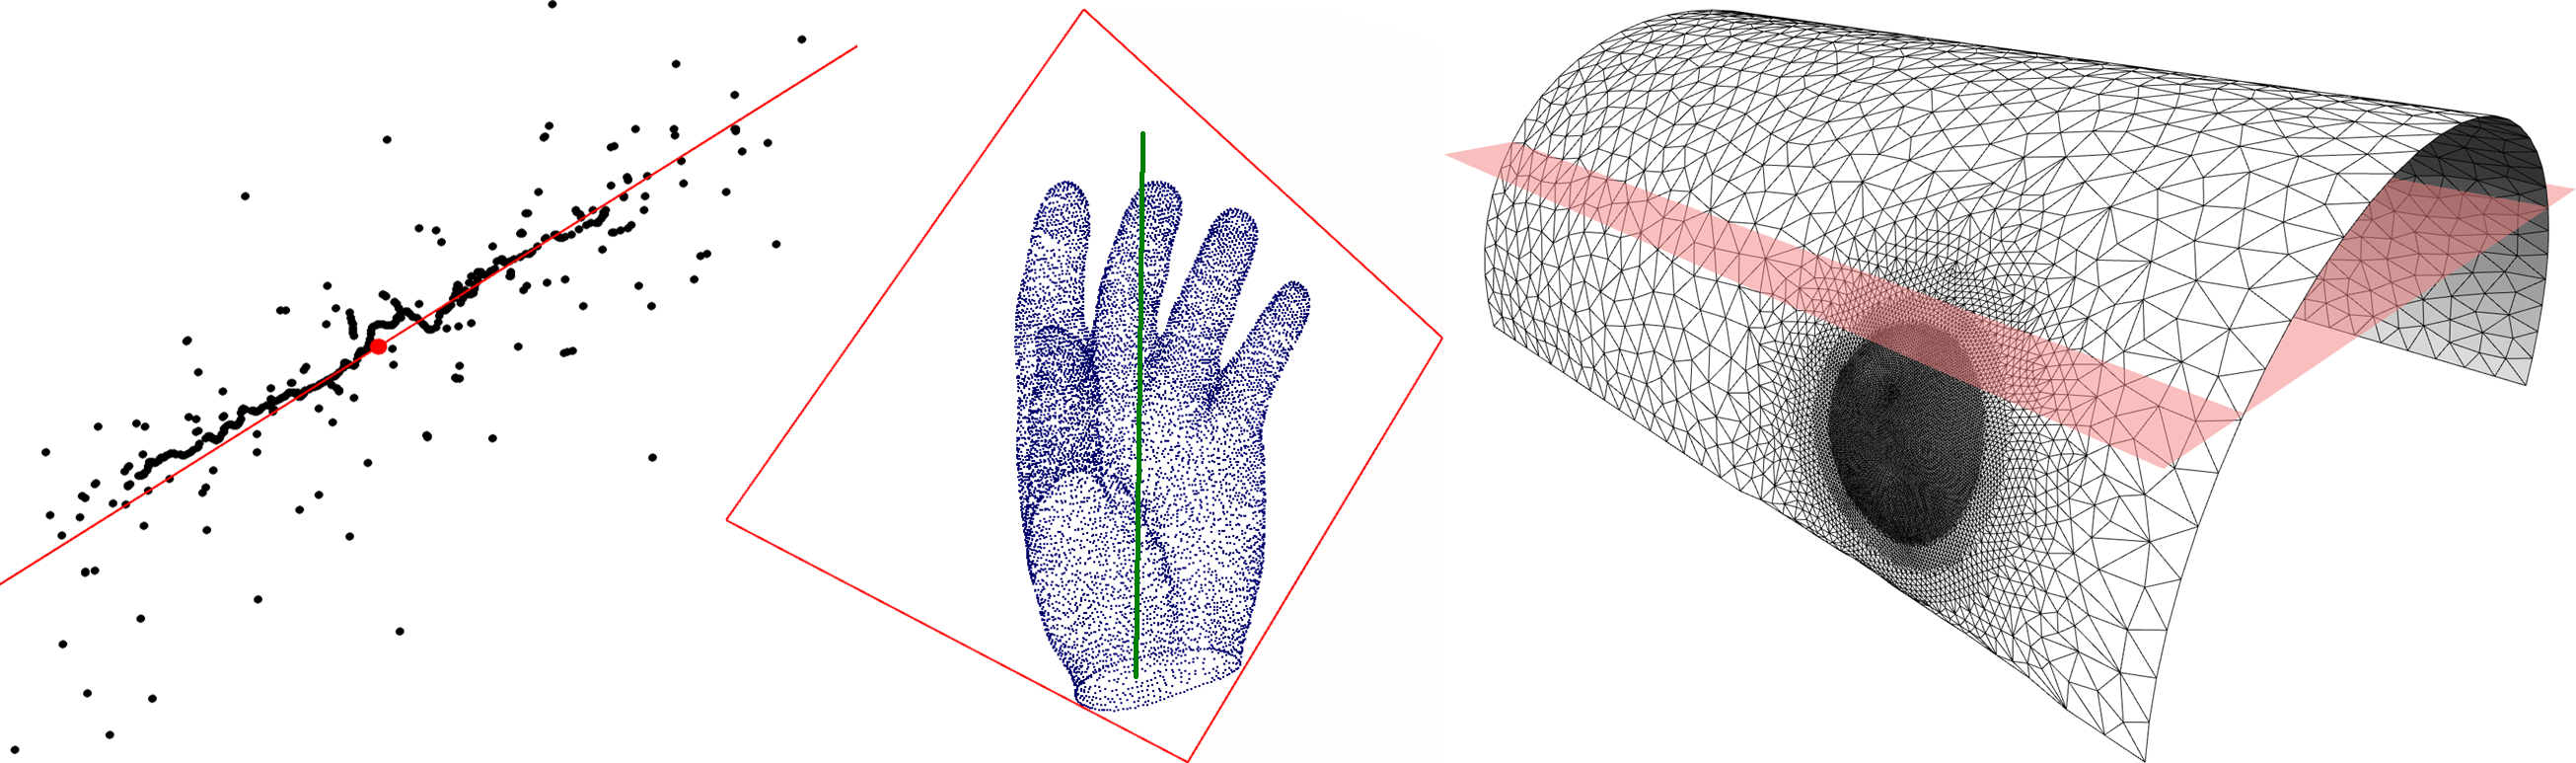
\includegraphics[width=1.0\textwidth]{Principal_component_analysis/fit}
    \end{ccTexOnly}
    \begin{ccHtmlOnly}
        <img width="100%" border=0 src="./fit.png"><P>
    \end{ccHtmlOnly}
    % Title
    \begin{figure}[h]
        \caption{Left: fitting a line to a 2D point set.
                 Right: fitting a line and a plane to a 3D point set.}
    \end{figure}
\end{center}

